\documentclass[11pt]{article}
\usepackage{float}
\begin{document}
\title{7-1 Meeting Outline}
\maketitle
\section{Data Source}
The data we used in this simulation is a time-series data of monthly retail sales from 01/01/1992 to 05/01/2016.
\begin{figure}[H]
\centering
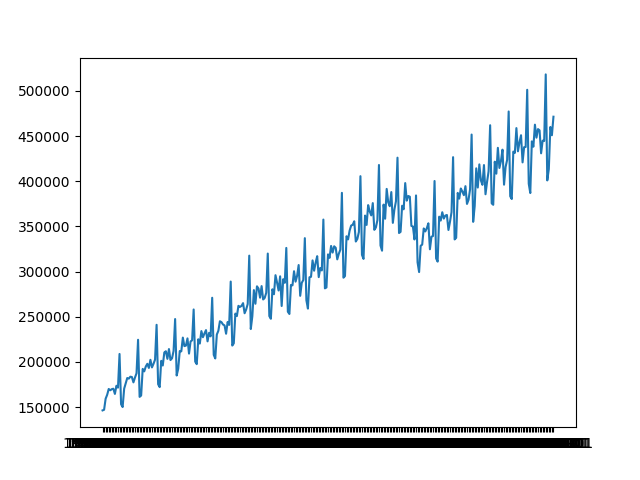
\includegraphics[scale=1]{./data_diagram.png}
\end{figure}

\section{Bayesian Agent}
Our data are divided into two parts. The first part is prior data, which are fed into agents to form their prior beliefs. The prior is formed by $n$ and $\niu$. $n$ is the number of prior data fed into the agent. $\niu$ is the mean value of the prior data agent has. And once agent enters the market, he would update his signal based on both prior data and $m$ data before he enters. The update rule is:
$$
\niu=\frac{n*\niu+m*\hat{mu}}{n+m}
$$
$\niu$ is the agent's private signal. When deciding the amount of shares he should sell or purchase, the agent would also take current price in to account. His belief is formed by

$$
\frac{n\niu+\hat{\mu}}{n+1}
$$

,where $n$ is the number of trades posted by the market maker, $\niu$ is the current price, $\hat{\mu}$ is agent's private signal.

The agent can calculate $\delta$ based on the cost function and his belief by 

$$
\Delta C(\theta+\delta)=\frac{n\niu+\hat{\mu}}{n+1}
$$
\end{document}
